\chapter{Background}\label{cha:background}
Maze has a long history spanning thousands of years. It intrigued ancient philosophers, artists, and scientists. In the modern days, we can easily say that mazes are everywhere.
From children's puzzles, traced by finger, pac-man game, psychology experiments on mice in a laboratory to the movie Labyrinth from 1986. But the omnipresence of mazes is even greater. 
Mazes also intrigued scientists who are still studying them carefully. It was soon noticed that it may also present the maze construction as a graph. Every problem which may be presented as a graph problem has the same laws as the maze. And so we discover an enormous variety of real-life applications of maze theory such as navigation systems, transportation route planning systems, building complexity in video games, solving networking and electrical problems and describing complex systems in physics and chemistry.
To its popularity, we can state with ease that studying the maze generating and solving algorithms, searching for difficulty measures, and searching for a new better solution for many real-life applications is important, both for amateurs, specialists, and society. In this chapter, I provide a theoretical background of maze-generating algorithms, maze-solving algorithms, and other theoretical concepts from the graph theory required to better understand the problems included in this paper. I will also present a background for determining the difficulty of a maze. 
\section{Graph Theory Theoretical Background}\label{sec:theoreticalBackground}
In the following section, I will discuss graph theory's most important mathematical concepts and establish a naming convention to follow in this paper. 
\begin{definition}\textbf{A Set} is an object of distinct elements where no element is a set itself.\end{definition}
\begin{definition}\textbf{A Graph}is an object comprising two sets called vertex set and edge set. The vertex set is a finite, nonempty set and the edge set may be empty. A graph usually denoted as $ G = (V, E)$ is a pair of a $V$ set of nodes (\textit{vertices}), and $E$ set of (\textit{edges}).. \end{definition}
In this paper, I will consider three interesting subgroups of graphs:
 \begin{itemize}
 \item[$-$] weighted graph,
 \item[$-$] directed graph,
 \item[$-$] cyclic graph.
 \end{itemize}
 \begin{figure}[!h]
	\centering
	\begin{subfigure}{.35\textwidth}
	  \centering
	  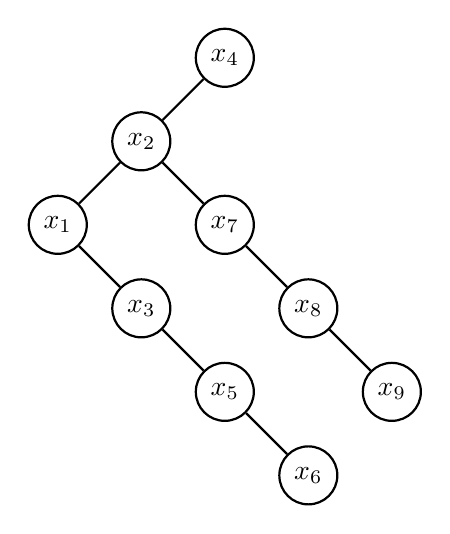
\begin{tikzpicture}[node distance={15mm}, thick, main/.style = {draw, circle}] 
		\node[main] (1) {$x_1$}; 
		\node[main] (2) [above right of=1] {$x_2$}; 
		\node[main] (3) [below right of=1] {$x_3$}; 
		\node[main] (4) [above right of=2] {$x_4$}; 
		\node[main] (5) [below right of=3] {$x_5$}; 
		\node[main] (6) [below right of=5] {$x_6$}; 
		\node[main] (7) [below right of= 2] {$x_7$};
		\node[main] (8) [below right of= 7] {$x_8$};
		\node[main] (9) [below right of= 8] {$x_9$};
		\draw (1) -- (2);
		\draw (2) -- (4);
		\draw (1) -- (3);
		\draw (3) -- (5);
		\draw (5) -- (6);
		\draw (2) -- (7);
		\draw (7) -- (8);
		\draw (8) -- (9);
		\end{tikzpicture} 
	  \caption{Graph of a maze in Figure 1.4(a)}
	  \label{fig:sub1}
	\end{subfigure}
	\begin{subfigure}{.35\textwidth}
	  \centering
	  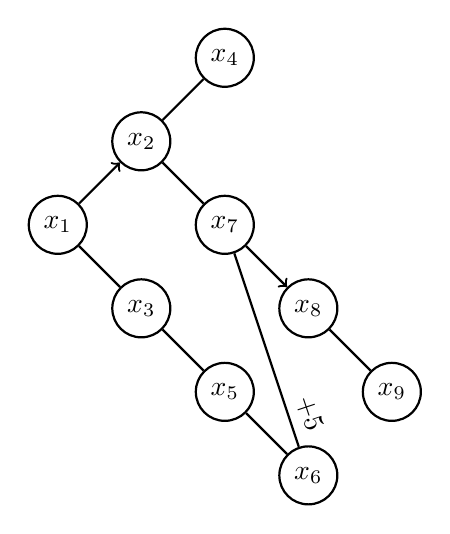
\begin{tikzpicture}[node distance={15mm}, thick, main/.style = {draw, circle}] 
		\node[main] (1) {$x_1$}; 
		\node[main] (2) [above right of=1] {$x_2$}; 
		\node[main] (3) [below right of=1] {$x_3$}; 
		\node[main] (4) [above right of=2] {$x_4$}; 
		\node[main] (5) [below right of=3] {$x_5$}; 
		\node[main] (6) [below right of=5] {$x_6$}; 
		\node[main] (7) [below right of= 2] {$x_7$};
		\node[main] (8) [below right of= 7] {$x_8$};
		\node[main] (9) [below right of= 8] {$x_9$};
		\draw[->] (1) -- (2);
		\draw (2) -- (4);
		\draw (1) -- (3);
		\draw (3) -- (5);
		\draw (5) -- (6);
		\draw (2) -- (7);
		\draw (6) -- node[midway, above left, sloped, pos=0] {+5} (7);
		\draw[->] (7) -- (8);
		\draw (8) -- (9);
		\end{tikzpicture} 
	  \caption{Graph of maze in Figure 1.4(b)}
	  \label{fig:sub2}
	\end{subfigure}
	\caption{A different types of graphs}
	\label{fig:test}
	\end{figure}

By applying \textit{weight} or \textit{direction} to edges, we are receiving a \textit{ weighted graph} or \textit{directed graph}. A cyclic graph consists of at least one single \textit{cycle}, which means at least 3 vertices connect in a closed chain. 
\newline
\begin{definition} \textbf{An Adjacency Matrix } of a graph $G=(V, E)$ is a representation in which we number the vertices in some arbitrary way e.g. $1,2,3,\dots, |V|$. The representation of a Matrix of
consisting $|V|x|V|$ such that: 
$$A(i,j)=
\begin{cases}
1, if (i,j)\in E,\\
0, otherwise\\
\end{cases}$$
Figures 1.2(a) and 1.2(b) are the adjacency matrices of the undirected and directed graphs.
The adjacency matrix of a graph requires $\varTheta(V^2)$ memory, independent of the number of edges in the graph.
\end{definition}
\begin{figure}[!h]
	\centering
	\begin{subfigure}{.35\textwidth}
	  \centering
	  $\begin{pmatrix}
		0&1&1&0&0&0&0&0&0\\
		1&0&0&1&0&0&1&0&0\\
		1&0&0&0&1&0&0&0&0\\
		0&1&0&0&0&0&0&0&0\\
		0&0&1&0&0&1&0&0&0\\
		0&0&0&0&1&0&0&0&0\\
		0&1&0&0&0&0&0&1&0\\
		0&0&0&0&0&0&1&0&1\\
		0&0&0&0&0&0&0&1&0\\
	\end{pmatrix}$
	  \caption{An adjacency matrix of an undirected, unweighted, acyclic maze}
	  \label{fig:sub1}
	\end{subfigure}
	\begin{subfigure}{.35\textwidth}
	  \centering
	  $\begin{pmatrix}
		0&1&1&0&0&0&0&0&0\\
		0&0&0&1&0&0&1&0&0\\
		1&0&0&0&1&0&0&0&0\\
		0&1&0&0&0&0&0&0&0\\
		0&0&1&0&0&1&0&0&0\\
		0&0&0&0&1&0&5&0&0\\
		0&1&0&0&0&0&0&1&0\\
		0&0&0&0&0&0&0&0&1\\
		0&0&0&0&0&0&0&1&0\\
	\end{pmatrix}$
	  \caption{An adjacency matrix of a weighted, directed, cyclic maze}
	  \label{fig:sub2}
	\end{subfigure}
	\caption{Examples of different adjacency matrices:}
	\label{fig:test}
\end{figure}

	\newpage
	\begin{definition} \textbf{A Graph} in which all vertices are adjacent to all others is said to be complete. \end{definition}
	\begin{definition} \textbf{Density} of a graph defines how complete the graph is. We define density as the number of edges divided by the number called \txtit{possible}. The number of possible is the maximum number of edges that the graph can contain.
	If self-loops are excluded, then the number possible is:\\
	\begin{equation}\label{acyclic_density}
	\frac{n(n-1)}{2}
	\end{equation}
	\textbf{Where:}\\
	$n$ is the number of vertices in a graph.\\
	\newline
	If self-loops are allowed, then the number possible is:
	\begin{equation}\label{cyclic_density}
	\frac{n(n+1)}{2}
	\end{equation}
	\textbf{Where:}\\
	$n$ is the number of vertices in a graph.
	\newline
	\end{definition}
\begin{definition}\textbf{A Free Tree} is an undirected, acyclic, connected graph. Let $G = (V,E)$ be an undirected graph. The following properties of a tree apply \\
\begin{itemize}
	\item[$-$] \textit{G} is a free tree,
	\item[$-$] every two nodes in \textit{G} are connected by a unique path,
	\item[$-$] \textit{G} is connected, but if any edge is removed from \textit{E},the graph becomes disconnected,
	\item[$-$] \textit{G} is connected, and $|E| = |V| - 1$,
	\item[$-$] \textit{G} is acyclic, and $|E| = |V| - 1$
	\item[$-$] \textit{G} is acyclic, but if we add any edge to \textit{E}, the graph contains a cycle. 
	\end{itemize}
\end{definition}
\begin{definition}\textbf{A Binary Tree} is a tree in which each node has no more than two subordinate nodes. Is composed of three disjoint sets of nodes: a root node, a binary tree called its left subtree, and a binary tree called its right subtree.\end{definition}
\begin{definition}\textbf{A Spanning Tree }\textit{T} is an acyclic tree which connects all the vertices in the graph \textit{G}. The minimum-spanning problem is a problem of determining the tree \textit{T} whose total weight is minimized.\end{definition}
\begin{definition}\textbf{A Path }in a graph $G$ is a sequence of nodes $v_1, v_2,\ldots,v_k$. The shortest path is a path with the lowest cost between any two given nodes.\end{definition}
\begin{definition}\textbf{A Shortest Path Problem }is finding for a given graph $G = (V,E)$, a shortest path from any 2 given nodes \textit{u} to \textit{v}. Shortest-paths algorithms typically rely on the property that a shortest path between two vertices contain other shortest paths within it.
The shortest path cannot contain any cycles.\cite{RTrud}\end{definition}
\begin{definition}\textbf{A Cell} is a single node in the maze matrix. The position of a cell is given by its id eg. for a cell with a position $a_{11}$ in a grid, we will note the id as $"1\char"0023 1"$; Is also the smallest element of the maze. The cell keeps the following information: its coordinates, the number of neighbours and their’s position relative to the cell.	\end{definition}
\begin{definition}\textbf{A Degree }of a vertex is denoted as $d(v)$ and it describes the number of adjacent cells.\cite{ReHofs}\end{definition}
\begin{definition}\textbf{An Average Degree } $\bar{d}$ for a given graph is given by \cite{ReHofs}:\\
\begin{equation}
\bar{d} = \frac{density}{n-1}	
\end{equation}
\textbf{Where:}\\
$n$ is a number of nodes in the graph\\	
\end{definition}
\begin{definition}\textbf{A Dead End} is defined as a node with a degree $d(v) = 1$. In the maze it's a cell that is linked to only one adjacent node.\end{definition}
\begin{definition}\textbf{A Fork} is defined as a node with a degree $d(v) = 2$. In the maze it's a cell that is linked to two adjacent nodes.\end{definition}
\begin{definition}\textbf{An Intersection} is defined as a node with a degree $d(v) = 3$. In the maze it's a cell that is linked to three adjacent nodes.\end{definition}
\begin{definition}\textbf{A Cross} is defined as a node with a degree$d(v) = 4$. In the maze it's a cell that is linked to four adjacent nodes. \end{definition}
\begin{definition}\textbf{A Grid} in this paper is considered as a square matrix. Its size defines the size of a maze $n \times n$. The grid keeps the information about each cell and their relative positions in an array.\end{definition}
\begin{definition}\textbf{A Move} is considered as a transition from one cell to one of its closest neighbours. In this paper, we are using only NSWE moves presented in Figure 1.3. Diagonal moves are forbidden.
\newline
\begin{figure}[!h]
	\centering
	\includegraphics[width=.2\linewidth]{moves}
	\caption{Allowed moves}
\end{figure}		
\end{definition}
\newpage
\begin{definition}\textbf{A Maze} can be considered as a graph, where each intersection is a vertex, and the path between them is an edge. \end{definition}
In this paper, I will be considering only 2D mazes on a rectangular grid Figure 1.1. The grid during the implementation process will be treated as a graph Figure 1.1. I will consider a few types of mazes:
 \begin{itemize}
 \item[$-$] perfect maze,
 \item[$-$] directed maze,
 \item[$-$] cyclic maze.
 \end{itemize}
 The perfect maze will be a maze with only one path between any two given nodes, a directed maze will be a maze with some paths directed in a certain direction, and a cyclic maze will be a maze with at least one cycle. 
 \newline
 \begin{figure}[!h]
	\centering
	\begin{subfigure}{.45\textwidth}
	  \centering
	  \includegraphics[width=.6\linewidth]{undirected_maze}
	  \caption{An undirected, unweighted, acyclic maze}
	  \label{fig:sub1}
	\end{subfigure}
	\begin{subfigure}{.45\textwidth}
	  \centering
	  \includegraphics[width=.6\linewidth]{cyclic_maze}
	  \caption{A weighted, directed, cyclic maze}
	  \label{fig:sub2}
	\end{subfigure}
	\caption{Examples of different mazes}
	\label{fig:test}
	\end{figure}
	\newline
If not mentioned otherwise, we assume the start and goal position to always be in the upper-left and lower-right, respectively Figure 1.4.
\newline	
 \begin{definition}\textbf{A Texture} is a general term that refers to the style of the passages of a maze, such as how long they tend to be and which direction they tend to go. Some algorithms will tend to produce mazes that all have similar textures.\cite{mazes}\end{definition}

 Binary Tree, for example, will always produce mazes with those two unbroken corridors on the north and east.
\begin{definition}\textbf{A Canadian Traveller Problem (CTP)} is a problem of finding the shortest path in a given, known graph with changing conditions in it. The objective of this problem is to find the best solution in the environment which is interfering with malicious intention.\end{definition}
\begin{definition}\textbf{A Travelling Salesman Problem (TSP)} is a problem of finding the shortest path between a given list of nodes in the graph. \end{definition}

\section{Maze Generation Algorithms}
\subsection{Binary Tree}
The Binary Tree algorithm is the simplest algorithm for generating a maze. In a given grid, for each cell algorithm decides whether to carve a passage north or east (or any two other directions south/west, south/east etc. ) between two adjacent cells. The algorithm produces a diagonally biased perfect maze which, in other words, is a random binary tree. For building the whole maze, the algorithm doesn’t require holding the state of the whole grid. The algorithm only looks at one cell at a time. The time complexity for the Binary Tree generator is $O(|V|)$. Below pseudocode for a Binary Tree algorithm.
\newline
\begin{lstlisting}[caption={Pseudocode for a Binary Tree Algorithm}]
\begin{algorithm}
\FOREACH cell in the grid
	\STATE let neighbours = [];
	\STATE neighbours.push(cell.north);
	\STATE neighbours.push(cell.east);
	\STATE let index = Math.floor(Math.random() * neighbors.length);
	\STATE let neighbor = neighbors[index];
	\STATE cell.link(neighbor);
\ENDFOREACH	
\end{algorithm}
\end{lstlisting}
\\
\newline
\begin{figure}[!h]
	\centering
	\begin{subfigure}{.45\textwidth}
	  \centering
	  \includegraphics[width=.6\linewidth]{binary1010}
	  \caption{Binary Tree maze 10 $\times$ 10}
	  \label{fig:sub1}
	\end{subfigure}
	\begin{subfigure}{.45\textwidth}
	  \centering
	  \includegraphics[width=.6\linewidth]{binary2020}
	  \caption{Binary Tree maze 20 $\times$ 20}
	  \label{fig:sub2}
	\end{subfigure}
	\caption{Examples of different binary tree mazes}
	\label{fig:test}
	\end{figure}

\subsection{Aldous-Broder}

The Aldous-Broder is a well-known algorithm for generating uniform spanning trees (USTs) based on random walks. This means that the maze is perfect and unbiased \cite{INune}. In a given grid, the algorithm randomly chooses any cell, and for this cell randomly chooses a neighbour and if this neighbour wasn’t previously visited, the algorithm links it to the prior cell. It is repeated until every cell has been visited. To build a spanning tree, the random walk needs to visit every vertex of the graph at least once. The time complexity for the Aldous - Broder generator is $O(|V|^3)$. Below pseudocode for an Aldous- Broder algorithm.
\newline
\begin{lstlisting}[caption={Pseudocode for an Aldous-Broder algorithm}]
\begin{algorithm}
\STATE let cell = grid.get_random_cell();
\WHILE unvisited cell in the grid
	\STATE let neighbours = cell.neighbours
	\STATE let index = Math.floor(Math.random() * neighbours.length);
	\STATE let neighbour = neighbours[index];
	\IF neighbour has no links
		\STATE cell.link(neighbour);
	\ENDIF
	\STATE cell = neighbour;
\ENDFOREACH
\end{algorithm}
\end{lstlisting}

\newline
\begin{figure}[!h]
	\centering
	\begin{subfigure}{.45\textwidth}
	  \centering
	  \includegraphics[width=.6\linewidth]{aldous1010}
	  \caption{Binary Tree maze 10 $\times$ 10}
	  \label{fig:sub1}
	\end{subfigure}
	\begin{subfigure}{.45\textwidth}
	  \centering
	  \includegraphics[width=.6\linewidth]{aldous2020}
	  \caption{Binary Tree maze 20 $\times$ 20}
	  \label{fig:sub2}
	\end{subfigure}
	\caption{Examples of different aldous-broder mazes}
	\label{fig:test}
	\end{figure}

\subsection{Recursive Backtracker}

The Recursive Backtracker is one of the Depth First Search algorithm (DFS) which may be also used for generating mazes. It generates perfect mazes with a small ratio of dead ends in a maze. Its main disadvantage is that it requires a lot of memory, so it is not fast or efficient. The algorithm starts at the randomly selected cell and carves its way until it must “turn around” and backtracks to the nearest “not carved yet” cell. This process continues until we have discovered all the vertices that are reachable from the source vertex. The time complexity for the Recursive-Backtracker generator is $O(|V|+|E|)$. Below pseudocode for a Recursive-Backtracker algorithm.

\begin{lstlisting}[caption={Pseudocode for a Recursive-Backtracker algorithm}]
	\begin{algorithm}
	\STATE let cell = grid.get_random_cell();
	\STATE let stack = [cell]
	\WHILE stack.length > 0
	\STATE let current_cell = stack[stack.length - 1];
	\STATE let neighbors = current.neighbors();
		\IF neighbors.length == 0
			\STATE stack.pop()
		\ELSE 
			\STATE let neighbor = neighbors[Random]
			\STATE current.make_link(neighbor)
			\STATE stack.push(neighbour)	
	\end{algorithm}
	\end{lstlisting}
\newline
\begin{figure}[!h]
    \centering
    \begin{subfigure}{.45\textwidth}
    \centering
    \includegraphics[width=.6\linewidth]{recursive1010.png}
    \caption{Binary Tree maze 10 $\times$ 10}
    \label{fig:sub1}
    \end{subfigure}
    \begin{subfigure}{.45\textwidth}
    \centering
    \includegraphics[width=.6\linewidth]{recursive2020.png}
    \caption{Binary Tree maze 20 $\times$ 20}
    \label{fig:sub2}
    \end{subfigure}
    \caption{Examples of different recoursive-Backtracker mazes}
    \label{fig:test}
    \end{figure}
\section{Maze Solving Algorithms}
\subsection{Breadth-First Search Algorithm - BFS}
BFS is one of the simplest algorithms for searching a graph. As already mentioned, we can consider each maze as a graph, so from now on we will call 
BFS  a solving algorithm or simply a solver of a given maze. From graph theory, we can state that for a given graph $ G = ( V, E) $, and distinct source 
vertex $s$, BFS explores the edges of $G$ to ,,visit’ each vertex directly connected with $s$. The algorithm also produces a BFS tree with $s$ root that 
contains all reachable vertexes. The shortest path  between $s$ and any vertex $v$ in $G$ is a simple path in the BFS tree, that is, a path containing
the smallest number of edges \cite{TCorm}.
\subsection{Dijkstra Algorithm}
Dijkstra is a solving algorithm for single-source shortest-path problems. We can apply it on a weighted, directed graph $G=(V, E)$ with a constraint of no negative edges. 
It repeatedly chooses the closest vertex in $V-S$ to add to set S. 
Where \textit{S} is a set of vertices whose final shortest-path weights from the source \textit{s} have already been determined.
As the algorithm floods the graph, we say it uses a greedy strategy.
\newline
\\
\begin{lstlisting}[caption={Pseudocode for a Dijkstra’s algorithm}]
	\begin{algorithm}
	\STATE let distances = new Distances();
	\STATE let frontier = new Array();
	\WHILE unvisited cell in the grid
		\FOREACH linked cell in frontier
			\STATE linked_cell.distance = cell.distance +1;
			\STATE distances.set_cell(linked_cell);
			\STATE frontier.push(linked_cell);
	    \ENDFOREACH
	\RETURN distances;
	\end{algorithm}
	\end{lstlisting}

\subsection{A* Algorithm}
$A^*$ algorithm is one of the most powerful path-finding algorithm. It uses two functions derived from the previously described algorithms. $A^*$ combines the information that Dijkstra’s Algorithm uses, meaning choosing the nodes which are close to the starting point and implementing a new type of information which is heuristic meaning choosing nodes which are estimated to be close to the ending point. In the standard terminology used when considering A*, g(n) represents the exact cost of the path from the starting point to any vertex n, and h(n) describes the heuristic estimated cost from vertex n to the goal. In each loop, the algorithm minimizes the following function:
\begin{equation}
neighbour.f = neighbour.g + neighbour.h
\end{equation}
\textbf{Where:}
neighbour.g = q.g + distance between q and neighbour\\
is a sum of distances from the starting point to the current node, and the distance from the current node to a neighbour.	\\
\newline
Maze problems usually have a quick access to basic heuristic functions because of a graph implemented as a grid. In this paper, we will use a heuristic method: a Manhattan Distance. Because we are using only the NSWE moves in discussed mazes, the Manhattan Distance is the best solution.
Manhattan Distance from neighbour cell to end cell is given as a:
\begin{equation}
neighbour.h = |end\_cell.x - neighbour.x| + |end\_cell.y - neighbour.y|
\end{equation}
\begin{lstlisting}[caption={Pseudocode for a A* algorithm}]
	\begin{algorithm}
	\STATE let openlist = new Array();
	\STATE let closelist = new Array();
	\STATE let startcell = maze.startcell;
	\STATE let goalcell = maze.goalcell;
	\STATE startcell.set_g_score();
	\STATE startcell.set_f_score();
	\STATE openlist.push(startcell)
	\STATE let finished = false;
	\WHILE (!finished)
		\STATE let currentcell = openlist    
		.find_cell_with_lowest_fvalue();
		\STATE let neighbours = currentcell.get_links();
			\IF currentcell == goalcell
				finished = true;
				closelist.push(currentcell);
			\ELSE 
			\FOREACH neighbour => neighbours	
			\IF inEitherList(openlist, closelist)
				\STATE g_score = calulate_gscore(cell);
				\STATE f_score = calculate_fscore(cell);
				\STATE parent = setParent(cell);
				\STATE openlist.push(cell)
			\ENDIF
			closelist.push(currentcell);
			openlist.remove(currentcell);
	    	\ENDFOREACH
	\end{algorithm}
	\end{lstlisting}

